\section{Auswertung}
\label{sec:Auswertung}
\subsection{Charakteristik des Geiger-Müller-Zählrohrs}
\label{subsec:auscharak}
Die Messwerte die wie in Abschnitt \ref{subsec:charak} beschrieben, aufgenommen wurden sind in Tabelle \ref{tab:imps} aufgelistet worden.
In der Abbildung \ref{fig:imps} wurden diese grafisch aufgetragen.
Die Grafik wurde mit dem python Plugin matplotlib \cite{matplotlib} erstellt.
Dabei ergibt sich der Fehler der Werte aus $\Delta N = \sqrt{N}$.
In der Grafik  ist ebenfalls eine Ausgleichsgerade zu sehen.
Diese wurde mit dem python Plugin scipy \cite{scipy} erstellt.
Die Werte mit denen die Ausgleichsgerade berechnet wurden, sind dabei die Werte die das Plateau bilden.
Zur Bestimmung der Qualität des Zählrohrs wurde nun die Steigung des Plateaus mithilfe der zuvor genannten Ausgleichsgeraden angenähert.
Dazu wurde diese nach dem Muster 
\begin{equation*}
  f(x) = ax +b 
\end{equation*} 
erstellt.
Die Wert der Steigung $a$ und der Wert $b$ sind dabei
\begin{align*}
  a &= \SI{1.16(22)}{\frac{\text{Imp}}{\weber}} \\
  b &= \SI{9.58(11)e03}{\frac{\text{Imp}}{\second}}\\
\end{align*}
Die Fehler bei der Rechnung und allen folgenden wurden mit dem python Plugin uncertainties \cite{uncertainties} berechnet.
Dieses nutzt die Gausschen-Fehlerfortpflanzungsformel 
\begin{equation*}
  \Delta y = \sqrt{\frac{\partial y}{\partial x_1}\Delta x_1+...}.
\end{equation*}

\begin{figure}
  \centering
  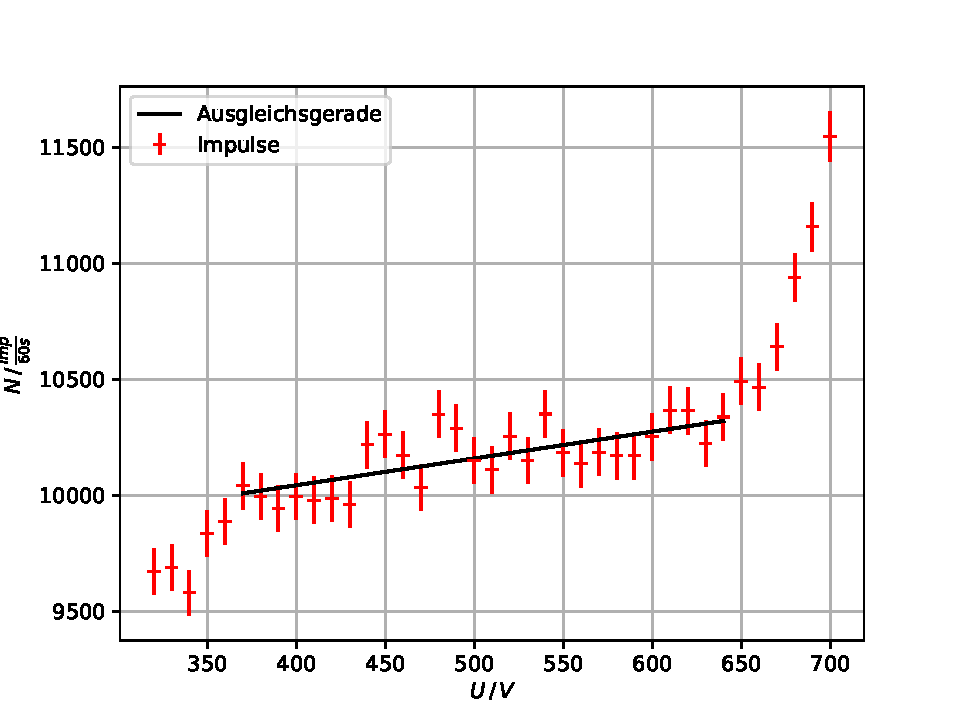
\includegraphics[width=0.6\textwidth]{content/data/kennlinie.pdf}
  \caption{Die aufgenommenen Messwerte mit zugehörigen Fehlern, sowie die Ausgleichsgerade im Plateau.}
  \label{fig:imps}
\end{figure}

\begin{table}
  \centering
  \caption{Die gemessenen Impulse pro $60\si{\second}$ in Abhängigkeit von der Spannung am Zählrohrs.}
  \begin{tabular}[t]{cc}
    \toprule
    $U \, /\, \si{\V}$ & $N \,/\, \frac{\text{Imp}}{\si{60\second}}$\\
    \midrule
    320 & 9672    \\
    330 & 9689    \\
    340 & 9580    \\
    350 & 9837    \\
    360 & 9886    \\
    370 & 10041   \\
    380 & 9996    \\
    390 & 9943    \\
    400 & 9995    \\
    410 & 9980    \\
    420 & 9986    \\
    430 & 9960    \\
    440 & 10219   \\
    450 & 10264   \\
    460 & 10174   \\
    470 & 10035   \\
    480 & 10350   \\
    490 & 10290   \\
    500 & 10151   \\
    510 & 10110   \\
    \bottomrule
  \end{tabular}
  \begin{tabular}[t]{cc}
    \toprule
    $U \, /\, \si{\V}$ & $N \,/\, \frac{\text{Imp}}{\si{60\second}}$\\
    \midrule
    520 & 10255   \\
    530 & 10151   \\
    540 & 10351   \\
    550 & 10184   \\
    560 & 10137   \\
    570 & 10186   \\
    580 & 10171   \\
    590 & 10171   \\
    600 & 10253   \\
    610 & 10368   \\
    620 & 10365   \\
    630 & 10224   \\
    640 & 10338   \\
    650 & 10493   \\
    660 & 10467   \\
    670 & 10640   \\
    680 & 10939   \\
    690 & 11159   \\
    700 & 11547   \\
    \bottomrule
  \end{tabular}
\label{tab:imps}
\end{table}
\FloatBarrier
\subsection{Totzeitberechnung}
Zur Berechung der Totzeit wurden die drei Werte
\begin{align*}
  N_1 &= \SI{96041}{\frac{\text{Imp}}{120\second}} \\
  N_{1+2} &= \SI{158479}{\frac{\text{Imp}}{120\second}} \\
  N_2 &= \SI{76581}{\frac{\text{Imp}}{120\second}} \\
  \label{eq:tot}
\end{align*}
aufgenommen.
Der Prozess der Messung ist in Abschnitt \ref{subsec:tot} beschrieben worden.
Mit diesen Werten kann mit Hilfe von Gleichung \eqref{eq:totzeit} die Totzeit $T$ des Geiger-Müller-Zählrohrs bestimmt werden.
Bei dem genutzten Zählrohr lässt sich die Totzeit auf 
\begin{align*}
  T = \SI{0.11(5)}{\milli\second}
\end{align*}
bestimmten.
Zudem wurde versucht die Totzeit durch ablesen an einem Osziloskop zu bestimmen.
Dies gelang nicht, da das Bild des Osziloskop unbrauchbar ist.
\FloatBarrier
\subsection{Freigesetzte Ladung pro eingefallenem Teilchen}
Zur Berechnung der Freigesetzte Ladung pro eingefallenem Teilchen wurde während der Messung der Impulse, in Abschnitt \ref{subsec:charak} beschrieben, auch die Stromstärke $I$ am Geiger-Müller-Zählrohr gemessen.
Die gemessenen Stromstärken sind in der Tabelle \ref{tab:strom} zusammen mit den jeweilgen Impulswerten zu sehen.
Aus diesen lassen sich mit der Gleichung \eqref{eq:z} die Zahl $Z$ berechnen, welche angibt wie viele Ladungen durch ein einfallendes Teilchen freigesetzt wurden.
Aus den berechneten Werten wurde im folgenden ein Plot erstellt, dieser ist in Abbildung \ref{fig:z} zu sehen.
Die Regressionsgerade wurde nach dem Schema $f(x)=ax+b$ erstellt.
Der Wert der Steigung $a$ entspricht dabei der gesuchten Zahl $Z$.
Die Werte für $a$ und $b$ entsprechen
\begin{align*}
  a &= \SI{3.24(14)e+16}{} \\
  b &= \SI{3.0(15)e+15}{}
\end{align*}
Also entspricht die Freigesetzte Ladung pro eingefallenem Teilchen $Z = \SI{3.24(14)e+16}{}$.

\begin{table}
  \centering
  \caption{Die gemessenen Stromstärken zu den passenden Impulswerten.}
  \begin{tabular}[t]{cc}
    \toprule
    $I \, /\, \si{\A}$ & $N \,/\, \frac{\text{Imp}}{\si{60\second}}$\\
    \midrule
    0.3 & 9837 \\
    0.4 & 9995 \\
    0.7 & 10264 \\
    0.8 & 10151 \\
    1.0 & 10184 \\
    1.3 & 10253 \\
    1.4 & 10493 \\
    1.8 & 11547 \\
    \bottomrule
    \end{tabular}
  \label{tab:strom}
\end{table}

\begin{figure}
  \centering
  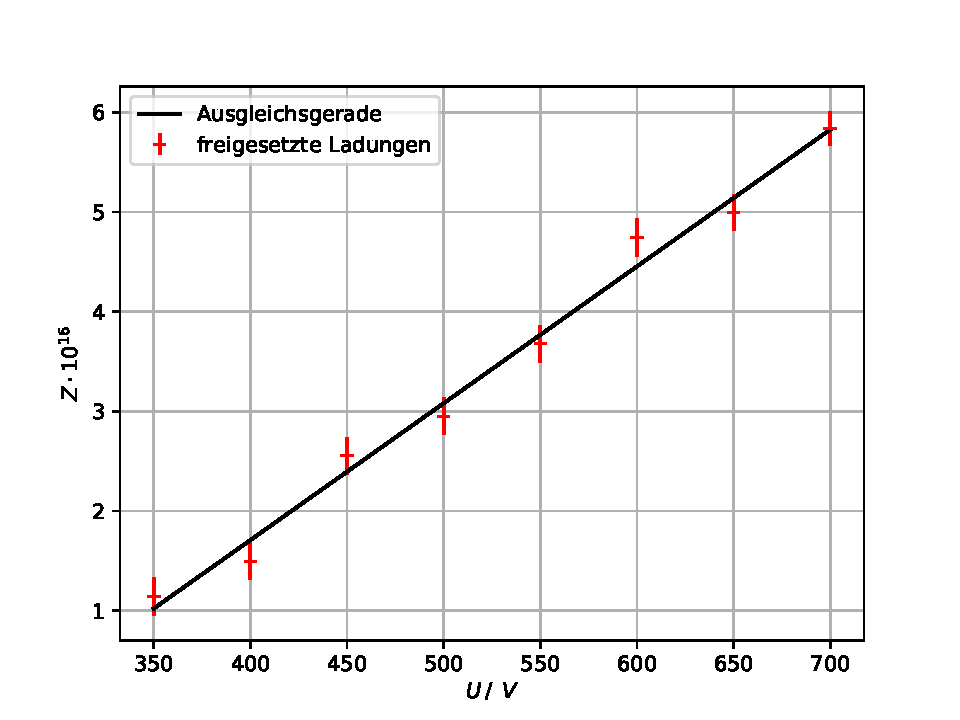
\includegraphics[width=0.6\textwidth]{content/data/zaehlstrom.pdf}
  \caption{Die Zahl der freigesetzten Ladungen pro Teilchen $Z$ aufgetragen gegen den Strom $I$.}
  \label{fig:z}
\end{figure}